\subsection*{الف}
در اینجا برای کشیدن زنجیره مارکوف می‌دانیم هر حالت با احتمال
$p$
به حالت بعد رفته و با احتمال
$1 - p$ 
به حالت قبل باز می‌گردد و این تا بی‌نهایت ادامه پیدا می‌کنید. به این ترتیب برای شکل این قسمت خواهیم داشت:
\begin{figure}[h]
    \centering
    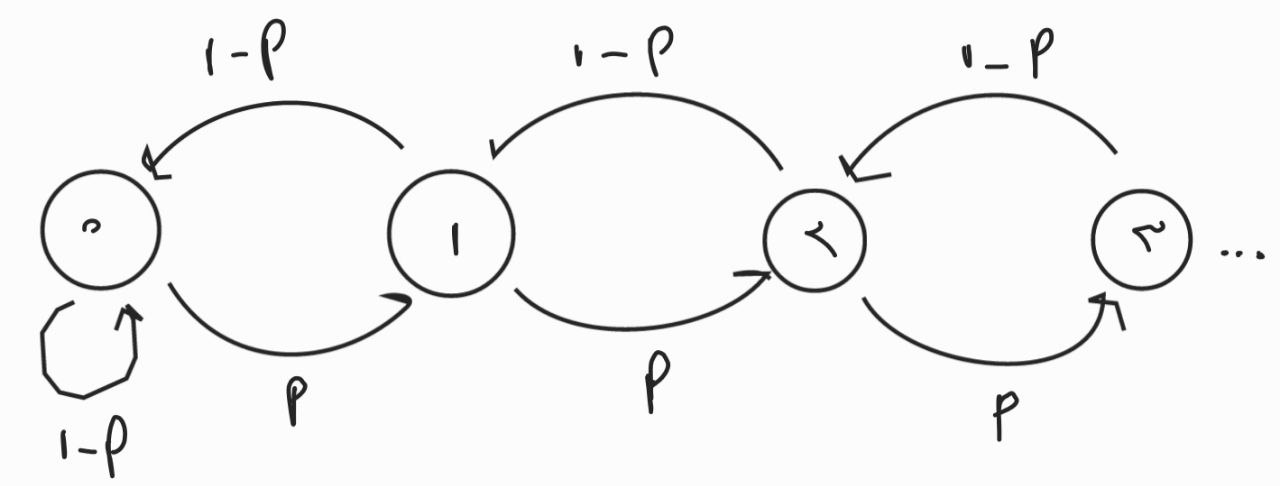
\includegraphics[scale = 0.3]{"commons/first.jpg"}
    \caption{شکل زنجیره مارکوف}
\end{figure}

\subsection*{ب}
برای محاسبه حالت ماندگار خواهیم داشت:
$$P_0 = (1 - p) P_0 + (1 - p) P_1 \implies P_1 = \frac{p}{1 - p} P_0$$
$$P_1 = p P_0 + (1 - p) P_2 \implies P_2 = \left(\frac{p}{1 - p}\right)^2 P_0$$
$$P_2 = p P_1 + (1 - p) P_3 \implies P_3 = \left(\frac{p}{1 - p}\right)^3 P_0$$
$$\implies P_i = \left(\frac{p}{1 - p}\right)^i P_0$$
حال باتوجه به جمع احتمالات
$P_i$
خواهیم داشت:
\begin{align*}
    \sum_{i = 0}^{\infty} P_i &= \sum_{i = 0}^{\infty} \left(\frac{p}{1 - p}\right)^i P_0 \\
                              &= \frac{P_0}{1 - \left(\frac{p}{1 - p}\right)} = 1, \quad p < 0.5
\end{align*}
$$ \implies P_0 = \frac{1 - 2p}{1 - p} \implies P_i = \left(\frac{p}{1 - p}\right)^i \left(\frac{1 - 2p}{1 - p}\right)$$
به این ترتیب احتمال وقوع هر حالت به این صورت خواهد بود.

\subsection*{ج}
با توجه به عبارات به دست آمده بالا می‌دانیم اگر داشته باشیم
$p > 0.5$
ضریب دنباله هندسی یعنی
$\frac{p}{1 - p}$
بزرگتر از یک خواهد شد و این نشان می‌دهد که جمع این دنباله به هیچ عنوان نمی‌تواند همگرا شود و نخواهیم داشت
$\sum_{i = 0}^{\infty} P_i = 1$.
به این ترتیب نمی‌توان برای احتمال وقوع حالت‌ها در این شرایط تعریفی بیان کرد.